\chapter{Clustering}\label{section-clustering}

The multi-input transaction clustering heuristic as introduced in section \ref{background:multi-input-tx} and as described in the paper 'A fistful of bitcoins...' \cite{Refworks:doc:5c3de7e3e4b0ea6196452d80} is one the most effective clustering heuristics for Bitcoin. In this section, we present the several implementations of clustering algorithms which uses the same input heuristic. We attempted clustering with many different approaches due to issues discovered while running each clustering algorithm. We also present the successful implementation in section \ref{clustering-raw-csv}.\todo{check this is accurate}

\section{The Algorithm}
The rough outline of the algorithm is shown below.
\begin{itemize}
    \item for each transaction $tx$ on the Blockchain
    \begin{itemize}
        \item Fetches inputs $ins$ of $tx$
        \item Gets all addresses $as$ where each $a$ in $as$ is an address which an input  $in$ from $ins$ is locked to
        \item Clusters the addresses $as$
    \end{itemize}
\end{itemize}

\section{Java \& Spring Data Approach}
The first approach taken was implemented as an extension of the Neo4J API 
\begin{itemize}
    \item Used the Spring Data interface to the database to fetch transactions from Neo4J
    \item For each transaction, make additional requests to Neo4J for inputs and addresses the inputs are locked to
    \item When a transaction has multiple inputs, add all addresses that input it to a set in memory 
    \item Execute a query to create a new relationship between every address in the set (such that it creates a totally connected sub-graph containing the addresses)
\end{itemize}
Executing this algorithm for a local instance of the database, which contained a subset of the Bitcoin Blockchain data (blocks 0-2000 only). The algorithm successfully completed and screenshots of the resulting database, with the new relationships introduced, can be seen in figure \ref{fig:neo4j-many-heuristic-1-clusters} and \ref{fig:neo4j-1-tx-heuristic-1-cluster}. 

\begin{figure}[h!]
  \centering
  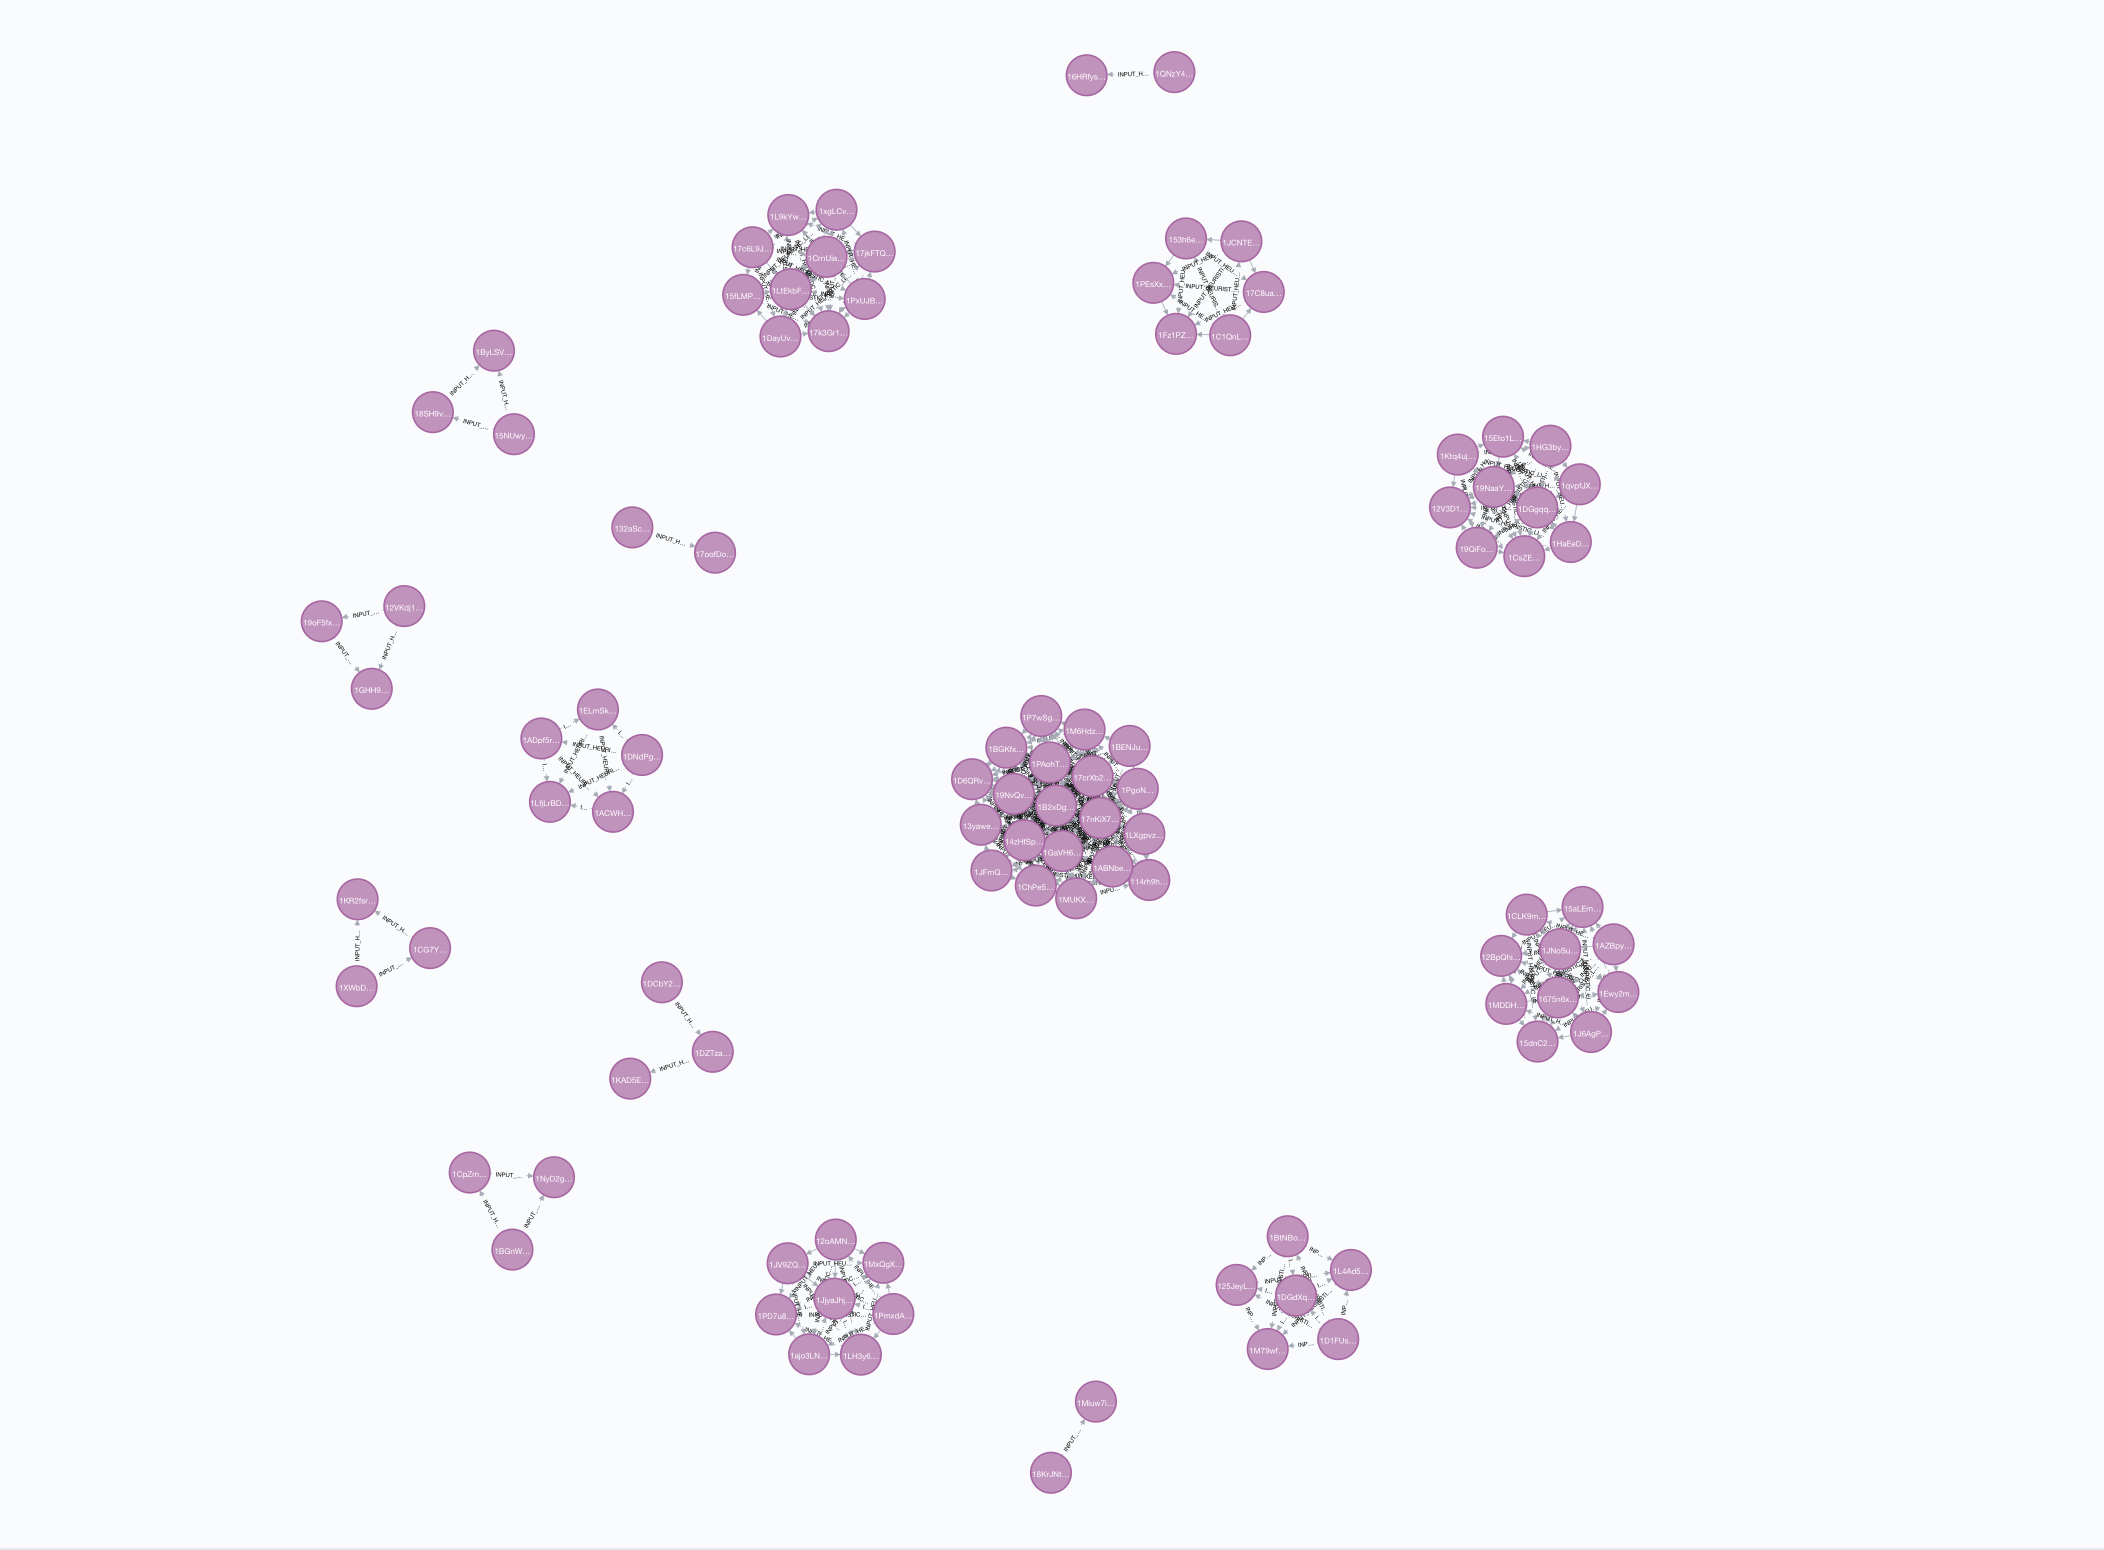
\includegraphics[width = 10cm]{./figures/many-clusters-heuristic-1}\\[0.5cm] 
  \caption{Neo4J browser view of the several clusterings of addresses which all feed the same transaction.}
  \label{fig:neo4j-many-heuristic-1-clusters}
\end{figure}

\begin{figure}[h!]
  \centering
  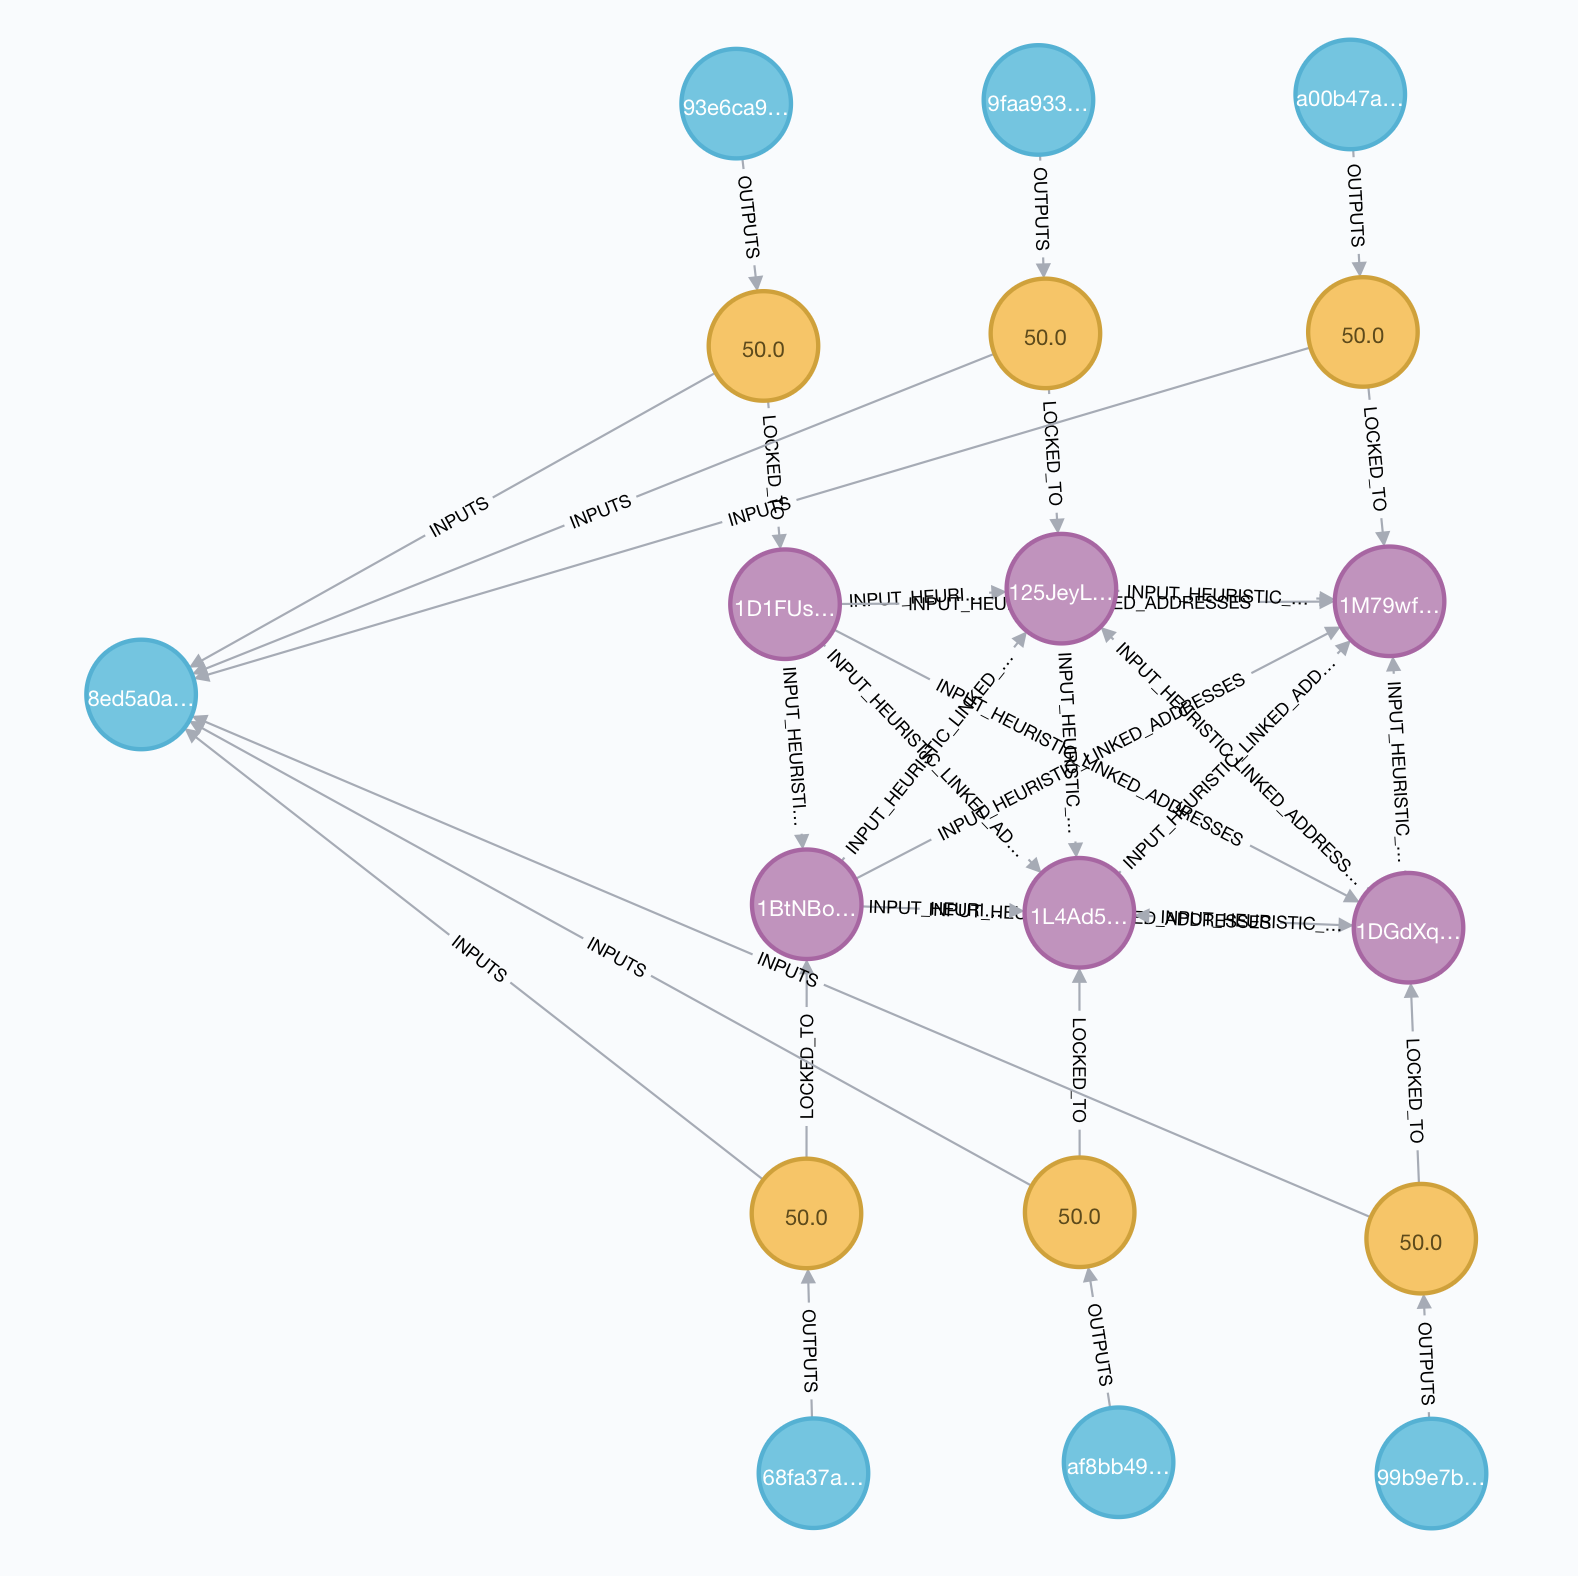
\includegraphics[width = 10cm]{./figures/input-one-tx-heuristic-1}\\[0.5cm] 
  \caption{Neo4J browser view one one of the clusterings of addresses with their neighbours expanded to show they all have outputs locked to them which feed the same transaction}
  \label{fig:neo4j-1-tx-heuristic-1-cluster}
\end{figure}


\subsection{Challenges}

An issue we anticipated would occur was an issue due to to the size of the dataset we are working with; we encountered a memory overflow error while the algorithm was attempting to load transactions in Bitcoin into memory. 
\\\\
We solved this issue using Paging. It is possible using Spring Data to use Paging for large requests; we used this to fetch transactions in batches, such that each batch's transactions could first be processed before fetching the next batch. This helped tackle memory constraints as the algorithm didn't need to load \textbf{all} transactions up front. See code in Listing \ref{lst:clustering-java}
\\\\
Although progress was now being made more steadily using paging, we still experienced performance issues while trying to cluster all addresses for the blockchain. After running the above algorithm for 24 hours, only 150,000 transactions had been processed. This was infeasibly slow, most likely due to the overhead of using Spring Data writing back new relations between each clustered address; it was clear a more efficient implementation was required.
\\\\

\begin{lstlisting}[caption={Java Implementation using Paging}, label={lst:clustering-java}, language=Java, breaklines=true, basicstyle=\small]
public ResponseEntity clusterByInput() {
    //Pageable item: start at page 0, fetch 50 items
    Pageable pageable = PageRequest.of(0, 50);

    while (true) {
        //Fetches transactions for this page
        Page<Transaction> allTransactions = transactionRepository.findAll(pageable);
        allTransactions.forEach(transaction -> {
            
            if (transaction.getInputs() == null || transaction.getInputs().size() < 2) {
                //coinbase input or only one input
                return;// just skips this iteration only
            }
            //Fetch inputs for this transaction
            List<InputRelation> transactionInputs = transaction.getInputs();
            Set<Address> addressesSpendingTransactionInputs = new HashSet<>();

            transactionInputs.forEach(inputRelation -> {
                String inputId = inputRelation.getInput().getOutputId();
                
                //Fetches the entire Output node from the database, so it's
                //relation fields are populated
                Output refetchedTransactionInput = getOutputById(inputId);
                Address addressSpendingTransactionInput = refetchedTransactionInput.getLockedToAddress();
                
                //add every distinct address to a set
                if (addressSpendingTransactionInput != null) {
                    addressesSpendingTransactionInputs.add(addressSpendingTransactionInput);
                }
            });

            //iterate through the set, link every item in set with evrey other
            addressesSpendingTransactionInputs.forEach(address -> {
                address.setInputHeuristicLinkedAddresses(addressesSpendingTransactionInputs);
                
                // Saves the updated addresses back to Neo4J repo at depth 0
                this.addressRepository.save(address, 0);
            });

            System.out.println("completed for tx" + transaction.getTransactionId());

        });

        if (!allTransactions.hasNext()) {
            //reached the last page: terminate
            break;
        }
        
        //fetches the next page to request
        pageable = allTransactions.nextPageable();
    }

    return ResponseEntity.status(200).body("Clustering Complete");
}
\end{lstlisting}

\section{Cypher Query}
The intention behind this implementation was if we could fully specify the algorithm in Cypher, then Neo4J could potentially parallelise/optimise the workload more efficiently if it knows the entire algorithm up-front. We also hoped that using Cypher would improve performance by bypassing the necessity to interact with the database using Spring Data, which will be adding some overhead. 
\\\\
We were able to translate the above algorithm in Listing \ref{lst:clustering-java} to a single Cypher query. The Cypher implementation is shown in Listing \ref{lst:clustering-cypher}.
The query matches all transactions that have more than one input, then finds the addresses each input is locked to. It uses the \texttt{UNWIND} commands to generate all pairs of addresses in the address list for a particular transaction. The clause \texttt{WHERE id(first) \< id(second)} ensures a pair of addresses only occurs once; rather than two pairs existing for \{a,b\} and \{b,a\} where a and b are both addresses.

\begin{lstlisting}[caption={Cypher Implementation}, label={lst:clustering-cypher}, breaklines=true, basicstyle=\small]
MATCH (t:TRANSACTION)
WHERE size((t)<-[:INPUTS]-()) > 1
WITH [(t)<-[:INPUTS]-(:OUTPUT)-[:LOCKED_TO]->(a:ADDRESS) | a] as addresses
UNWIND addresses as first
UNWIND addresses as second
WITH addresses, first, second
WHERE id(first) < id(second)
MERGE (first)-[:INPUTS_SAME_TX]-(second)
\end{lstlisting}

Before we could execute the query, we first had to clean up the mutations made to the database by running earlier clustering implementations. To do this, we created a Query to delete all instances of the relationships we added during the first attempt. 
\begin{lstlisting}
MATCH (:ADDRESS)-[r:INPUT_HEURISTIC_LINKED_ADDRESSES]-(:ADDRESS)
DELETE r
\end{lstlisting}

\subsection{Performance Issues}
When executing the query shown in Listing \ref{lst:clustering-cypher} we encountered performance issues where several hours would elapse with no apparent progress being made. 
\\\\
We investigated this issue using the Cypher \texttt{PROFILE} command to inspect the performance of this query. The performance report identified issues in the earlier stages where the query would require the search of all nodes across the database when matching transactions, inputs and addresses. Since we want to match all nodes, rather than using a specific ID that can leverage fast index lookups, this leads to a significant bottleneck in the query. Furthermore, investigating the issue using the \texttt{htop} command on the Satoshi VM, we could see that core utilisation was extremely low (almost completely idle).
\\\\
The main difficulty with this approach is that executing a very expensive query becomes almost like a 'black-box' in that it is difficult to understand what Neo4J is doing, since using the Community edition there are not many logging options that can be used to help us.

\section{Clustering on demand}
This approach has the intention of tackling the performance issues by only performing clustering when and where it is required, rather than attempting to perform clustering for the entire Bitcoin Blockchain in advance. 
\\\\
By knowing exactly which address we want to perform the clustering for, and leveraging the performance enhancements provided by indexes on address, transactions and outputs when fetching them using their respective ID's, we were able to craft an algorithm to implement clustering on demand.
\\\\
This implementation heavily relied on Java 8 streams, specifically using parallel streams to introduce concurrency in the clustering process, increasing the efficiency of this operation; critical for an on-demand implementation. 
\\\\
The implementation of this algorithm led me to discover that my initial implementation (Listing \ref{lst:clustering-java}) was not correct. This heuristic is transitive, such that if addresses A and B input the same transaction, and B and C input the same transaction then A, B and C can all be considered as under the control of the same user. My implementation in Listing \ref{lst:clustering-java} does not take this transitivity into account. However, we ensured transitivity was encountered before in my on-demand clustering algorithm in Listing \ref{lst:clustering-on-demand}.

\begin{lstlisting}[language=Java, caption={Java Implementation of on demand clustering}, label={lst:clustering-on-demand}, breaklines=true, basicstyle=\small]
private void performInputClustering(Address addressNode, Date start, Date end) {
    Set<Address> linkedAddresses = transitiveInputClustering(addressNode, new HashSet<>(), start, end);
    addressNode.setInputHeuristicLinkedAddresses(linkedAddresses);
}

private Set<Address> transitiveInputClustering(Address addressNode, Set<Transaction> exploredTransactions, Date start, Date end) {
    //a stream of transactions which all have inputs locked to this address
    Stream<Transaction> allTransactionsThisAddressInputs = getTransactionsForAddress(addressNode, start, end);
    HashSet<Transaction> thisAddressesTransactions = allTransactionsThisAddressInputs.collect(Collectors.toCollection(HashSet::new));

    //removes all transactions we've already seen
    thisAddressesTransactions.removeAll(exploredTransactions);

    //now adds the new transactions we're about to explore to the explored set
    exploredTransactions.addAll(thisAddressesTransactions);

    //all addresses linked directly (1 transaction hop away) from this address
    Stream<Address> linkedAddressesStream = getAddressesLinkedByTransactions(thisAddressesTransactions.parallelStream(), start, end);
    Set<Address> directlyLinkedAddresses = linkedAddressesStream.collect(Collectors.toSet());

    //all addresses linked transitively (2 transaction hops away) from this address
    Stream<Set<Address>> transitiveAddressStream = directlyLinkedAddresses
            .stream()
            .map(linkedAddress -> transitiveInputClustering(linkedAddress, exploredTransactions, start, end));
    directlyLinkedAddresses.addAll(transitiveAddressStream.flatMap(Set::stream).collect(Collectors.toSet()));

    return directlyLinkedAddresses;
}

private Stream<Transaction> getTransactionsForAddress(Address address, Date start, Date end) {
    return address.getOutputs()
            .parallelStream()
            .map(outputShell -> findOutputNode(outputShell.getOutputId(), start, end))
            .filter(outputNode -> outputNode.getInputsTransaction() != null)
            .map(outputNode -> outputNode.getInputsTransaction().getTransaction())
            .map(transactionShell -> findTransaction(transactionShell.getTransactionId()))
            .filter(transactionNode -> transactionNode.getInputs() != null && transactionNode.getInputs().size() > 1);
}

private Stream<Address> getAddressesLinkedByTransactions(Stream<Transaction> transactionStream, Date start, Date end) {
    return transactionStream.flatMap(tx -> getAddressesLinkedByTransaction(tx, start, end));
}
private Stream<Address> getAddressesLinkedByTransaction(Transaction transaction, Date start, Date end) {
    return transaction.getInputs()
            .parallelStream()
            .map(InputRelation::getInput)
            .map(inputShell -> findOutputNode(inputShell.getOutputId(), start, end))
            .map(Output::getLockedToAddress);
}
\end{lstlisting}

\subsection{Drawbacks \& Compromises}
On-demand clustering begins to become unsuitable for extremely large clusters; for example, an address belonging to the wallet of SatoshiDice.com \\\texttt{1LaM2aDLEP49kLbE6y2hvnbrP3agbMwEHb} would belong to an extremely large cluster of many thousands of addresses, and clustering on-demand would simply take far too long to provide an acceptable user experience (we experimented with the above address and killed the request after 30 minutes had elapsed). For addresses belonging to large wallets like the one above, we attempt to cluster using the entity tagging information obtained in section \ref{section-entity-tagging} rather than using the multi-input heuristic.
Since this data is stored in the database, it is quick to traverse the \texttt{HAS\_ENTITY} relationships from a known address to find all of the addresses in the cluster. Therefore, we prioritise providing entity clustering information over input clustering in order to provide as much valuable information over a shorter time; improving user experience. \\\\
For those addresses that do not have a link with a known entity, but exist as part of large address clusters, we truncate the search to a limit $N$ that is defined by the user. The user can increase and decrease this limit, including disabling it completely, when initiating the search [see more on this in section \ref{section-investigation-tool}]. Therefore, the algorithm will halt once $N$ addresses belonging to the cluster have been found. This is a trade-off between usability and utility; the truncation makes the feature more usable since it provides more reasonable response times, however it does not provide a complete result. The user can still obtain a complete result by disabling the limit, albeit at the risk of poor user experience. 

\section{Clustering using raw CSV data}\label{clustering-raw-csv}
The challenges experienced in previous implementations largely involved the necessity to write new relationships between addresses on a large scale to the database. If we were to circumvent this by calculating these relationships upfront before the bulk import into Neo4J, we would benefit from the powerful Neo4J Bulk Import tool making lighter work of writing these many relationships. 
\\\\
Once the relationships exist between clustered addresses in the graph, it will be efficient to query the database for addresses in the same cluster of a particular address;  Neo4J is designed to traverse a large number of relationships extremely quickly. 
\\\\

\subsection{Approach}
Each entry in the CSV file will have the format below where \texttt{ADDRESS\_IN\_CLUSTER} and \texttt{ANOTHER\_ADDRESS\_IN\_CLUSTER} are two Bitcoin addresses and \texttt{INPUTS\_SAME\_TX} is the name of the relationship. 

\begin{lstlisting}
ADDRESS\_IN\_CLUSTER, ANOTHER\_ADDRESS\_IN\_CLUSTER, INPUTS\_SAME\_TX
\end{lstlisting}

The outline of the algorithm is as follows:
\begin{itemize}
    \item for each transaction $tx$ on the Blockchain
    \begin{itemize}
        \item Fetches inputs $ins$ of $tx$
        \item Maps $ins$ to the addresses the input is locked to and generates a set of addresses $as$ which input the transaction 
        \item Writes a new CSV relationship entry for every pair $a1, a2$ in $as$ where $a1 != a2$
    \end{itemize}
    \item The new input relations CSV files are then used in the Neo4J import tool to re-import the entire database, now with clustering information
\end{itemize}
We leveraged concurrency in the implementation of the above algorithm. we implemented the algorithm in Java, splitting the transactions to be iterated through into separate chunks to be submitted to a pool of worker threads. We addressed possible race conditions and file lock contentions by having each thread writing to its own output CSV file.  